% -- %% ============================ Tufte' handout ===============================
% -- \documentclass[nobib]{tufte-handout}
% -- 
% -- %% ------------------------------ Tables -------------------------------------
% -- \usepackage{blkarray}          % convenient matrices
% -- \usepackage{rotating}          % rotate objects
% -- \usepackage{booktabs}          % book-quality tables
% -- \usepackage{units}             % non-stacked fractions and better unit spacing
% -- \usepackage{multicol}          % multiple column layout facilities
% -- \usepackage{lipsum}            % filler text
% -- \usepackage{fancyvrb}          % extended verbatim environments
% -- \fvset{fontsize=\normalsize} % font size for fancy-verbatim environments
% -- \usepackage{tabularx,ragged2e} % table formatting
% -- \usepackage{array}             % table formatting
% -- \usepackage{siunitx}           % alignment
% -- \sisetup{detect-all}
% -- \sisetup{input-symbols = ()}
% -- \usepackage{adjustbox}         % scaling
% -- \usepackage[T1]{fontenc}       % text
% -- \newcolumntype{P}[1]{>{\centering\arraybackslash}p{#1}}
% -- \usepackage{xcolor}            % coloured text etc.% 
% -- 
% -- %% --------- Standardize command font styles and environments ----------------
% -- \newcommand{\doccmd}[1]{\texttt{\textbackslash#1}}% adds backslash
% -- \newcommand{\docopt}[1]{\ensuremath{\langle}\textrm{\textit{#1}}\ensuremath{\rangle}}% optional command argument
% -- \newcommand{\docarg}[1]{\textrm{\textit{#1}}}% (required) command argument
% -- \newcommand{\docenv}[1]{\textsf{#1}}% environment name
% -- \newcommand{\docpkg}[1]{\texttt{#1}}% package name
% -- \newcommand{\doccls}[1]{\texttt{#1}}% document class name
% -- \newcommand{\docclsopt}[1]{\texttt{#1}}% document class option name
% -- \newenvironment{docspec}{\begin{quote}\noindent}{\end{quote}}% command specification environment
% -- 
% -- %% ----------------------------- Links ---------------------------------------
% -- \hypersetup{
% --     colorlinks=true,
% --     linkcolor=RoyalBlue,
% --     filecolor=RoyalBlue,      
% --     urlcolor=RoyalBlue,
% --     citecolor=Black,
% --     pdftitle={Overleaf Example},
% --     pdfpagemode=FullScreen,
% --     }
% --   
% -- %% -------------------------- Drawing and plots ------------------------------
% -- \usepackage{pgfplots}
% -- \pgfplotsset{compat=1.16}              % pgf plots
% -- \usepackage{pgf}
% -- \usepackage[utf8]{inputenc}\DeclareUnicodeCharacter{2212}{-}
% -- \usepackage{tikz}                      % tikz plots
% -- \usetikzlibrary{positioning}
% -- \usetikzlibrary{arrows.meta}
% -- \usetikzlibrary{backgrounds}
% -- \usetikzlibrary{calc}
% -- \usetikzlibrary{matrix}
% -- \usetikzlibrary{decorations.pathreplacing}
% -- \usetikzlibrary{fit}
% -- \def\firstcircle{(0,0) circle (1.5cm)} % custom shapes
% -- \def\secondcircle{(0:2cm) circle (1.5cm)}
% -- \colorlet{circle edge}{black!50}
% -- \colorlet{circle area}{black!20}
% -- \tikzset{filled/.style={fill=circle area, draw=circle edge, thick},
% -- outline/.style={draw=circle edge, thick}}
% -- \usepackage{tikz-network}
% -- \usepackage{sparklines}
% --   
% -- %% ----------------------------- Options -----------------------------------
% -- \usepackage{geometry}
% -- \renewcommand{\baselinestretch}{0.85}
% -- \usepackage{graphicx}          % allow embedded images
% --   \setkeys{Gin}{width=\linewidth, totalheight=\textheight, keepaspectratio}
% --   \graphicspath{{graphics/}}
% -- \usepackage{amsmath}                  % extended mathematics
% -- \usepackage[scaled=0.9]{helvet}       % sans-serif font to use
% -- \usepackage[defaultmathsize, symbolgreek]{mathastext}
% -- %\renewcommand\familydefault\sfdefault
% -- \Mathastext[helvet]
% -- \usepackage{sansmath}                 % maths with sans-serif
% -- \AtBeginEnvironment{tikzpicture}{\sansmath}
% -- \AtEndEnvironment{tikzpicture}{\unsansmath}
% -- \setsidenotefont{\sffamily\small}
% -- \setcaptionfont{\sffamily\small}
% -- \setmarginnotefont{\sffamily\small}
% -- \setcitationfont{\sffamily\small}
% -- 
% -- %% ----------------------------- Quotations ----------------------------------
% -- \usepackage{dirtytalk}
% -- 
% -- %% ------------------------------- Authors -----------------------------------
% -- \usepackage{authblk}
% -- 
% -- %% ----------------------------- References ----------------------------------
% -- %\usepackage[colorlinks, citecolor=DarkOrange]{hyperref}
% -- \usepackage[
% --   style=verbose,
% --   autocite=footnote,
% --   backend=biber,
% --   citestyle=authoryear
% -- ]{biblatex}
% -- \addbibresource{references/main_biblio.bib}
% -- \addbibresource{references/appendix_biblio.bib}

%% ============================ Classic wp ===================================
\documentclass[11pt]{article}

% ------------------------- Page and paragraph layout ------------------------
\usepackage[a4paper]{geometry}
\geometry{verbose,tmargin=1in,bmargin=1in,lmargin=1in,rmargin=1in}
%\setcounter{secnumdepth}{-2}
%\setcounter{tocdepth}{-2}
\usepackage{setspace}
\onehalfspacing%\doublespacing
\setlength{\parindent}{2.75em}
\setlength{\parskip}{1em}
%\renewcommand{\baselinestretch}{1.5}
\usepackage{titlesec}
\titlespacing{\section}{0pt}{1.5ex}{-1.5ex}
\titlespacing{\subsection}{0pt}{1.5ex}{-1.5ex}
\titlespacing{\subsubsection}{0pt}{1.5ex}{-1.5ex}
%\makeatletter
%\renewcommand{\@seccntformat}[1]{}
%\makeatother

%% -------------------------- Info on authors --------------------------------
\usepackage{authblk}

%% --------------------------- Text style ------------------------------------
\usepackage{color}

%% ----------------------------- Endnote -------------------------------------
%\usepackage{endnotes}
%\let\footnote=\endnote

%% ------------------------------- Links ------------------------------------- 
\usepackage[dvipsnames]{xcolor}
\usepackage[
	colorlinks=true,
	allcolors=base_c,
	%citecolor=CadetBlue,
	%urlcolor=CadetBlue
	]{hyperref}%
 
%% --------------------------- Bibliography ----------------------------------
\usepackage[
%natbib=true,
backend=biber,
style=alphabetic,
citestyle=authoryear,
%citestyle=apa,
%hyperref=true,
%maxbibnames=99,
%firstinits=false
maxcitenames=4,
%citetracker=true,
%parentracker=true,
bibstyle=authortitle
]{biblatex}

%% --------------------------- Exhibits --------------------------------------
\usepackage{array}
\usepackage{booktabs}
\usepackage{dcolumn}
\usepackage{pgfplots}
\pgfplotsset{compat=1.16}
\usepackage{pgf}
\usepackage[utf8]{inputenc}\DeclareUnicodeCharacter{2212}{-}
\usepackage{tikz}
%\usepackage{tabularx,ragged2e}
\usepackage{threeparttable}
\usepackage{graphicx}
\usepackage{rotating}
%\usepackage[T1]{fontenc}
%\usepackage{times}
%\usepackage{amsmath}
%\usepackage{mathptmx}
%\usepackage{bbm}
%\usepackage{dsfont}
%\usepackage{etoolbox}
\usepackage{caption}
\captionsetup[table]{labelfont=sc, labelsep=newline}
\renewcommand{\figurename}{Fig.}
%\usepackage{ctable}
\renewcommand{\thetable}{\Roman{table}}
\usepackage{csquotes}

% --------------------------- Appendices -------------------------------------
\usepackage[toc, page]{appendix}

% -------------------------- Tikz charts -------------------------------------
\definecolor{base_c}{HTML}{6A94D5}
\definecolor{comp_c}{HTML}{D5AB6A}
\definecolor{tri_1_c}{HTML}{D56A94}
\definecolor{tri_2_c}{HTML}{94D56A}
\definecolor{tet_1_c}{HTML}{D56ACA}
\definecolor{tet_2_c}{HTML}{D5AB6A}
\definecolor{tet_3_c}{HTML}{6AD575}

% -------------------------- References --------------------------------------
% load biblio
% ----------------------------------------------------------------------------
\addbibresource{references/main_biblio.bib}
\addbibresource{references/appendix_biblio.bib}

%% =============================== Document ==================================
%% ------------------------------ Cover page ---------------------------------
%% Title
\title{Exogenous Shocks in Leadership and Management Research:\\
Types, Challenges, and Opportunities\vspace{2em}}

%% Author
\author[$\bullet$]{Simone Santoni}
\author[$\star$]{Jost Sieweke}
\author[$\circ$]{Michael Withers}
\affil[$\bullet$]{Bayes Business School --- City, University of London}
\affil[$\star$]{Vrije Universiteit Amsterdam}
\affil[$\circ$]{Mays Business School --- Texas A\&M University}

\renewcommand\Authands{ and }
%\renewcommand\Authfont{\sffamily}
\renewcommand\Affilfont{\normalsize}

%% Date
\date{\vspace{1em} \normalsize \today \vspace{1em} \\ 
      \textcolor{red}{(Structured draft --- do not circulate)}}

%% ---------------------------- Body of the document -------------------------
\begin{document}

\begin{singlespace}

\maketitle

\begin{abstract}

---Abstract goes here---

\bigskip

\textit{Keywords}: kw1, kw2, kw3.

\end{abstract}

\end{singlespace}

\clearpage

\begin{refsection}[references/main_biblio.bib]

\section{Introduction}
\label{sec:introduction}

%% recall causal inference issues, mention attempts made by the community
% to improve causal inference, and connect these efforts with the popularity
% of natural experiments

The quest for empirical identification in management research has created
substantial attention around `natural experiments,' a form of causal inquiry
that has been traditionally popular in economics
\parencite[][]{Meyer1995,Rosenzweig2000} and political science
\parencite[][]{Dunning2008}.  The premise to conduct a natural experiment is the
presence of a `naturally' occurring event --- such as new regulations and laws,
natural disasters, or economic and political crises --- that heterogeneously
influences the units of a population \parencite[][]{Dunning2012,Robinson2009}.
Insofar as such event generates random or as-if random variations in the
environment, scholars can mimic the experimental ideal in which units are split
into a treatment and a control group or receive different levels of the
treatment. Ultimately, this opens up the possibility of inferring causal effects
when the substantive relationship at hand is difficult to investigate in a
laboratory setting and/or require operating costly, impractical, or unethical
field experiments.

% motivation for the article - NEs are not rooted in the field of strategic
% mangagement; rather, they are emerging as one of the most popular ways to
% tackle on the endogeneity challenge. As NEs diffuse in management research,
% pracrices emerge and crystallize on how to discover and leverage exogenous
% variations in order to test causal relationships. 

Although naturally occurring events can turn into opportunities to conduct
causal research, there are limited guidelines that help management scholars
prepare and review papers that implement the natural experiment research design.
To fill this gap, we highlight the strengths and weaknesses of natural
experiments as operated in the field of management studies and propose
actionable suggestions to assess and communicate the validity of natural
experiments.

To do so, we critically review the population of 147 natural experiments
published across seventeen top-tier management journals.\footnote{\todo{We're
updating the literature search on May 31, 2021.}} Our review aims
to address the following research questions: \emph{R1 --- How do management
scholars claim the random or as-if random nature of environmental variation at
the core of a natural experiment? R2 --- How do they claim the empirical and
substantive relevance of a natural experiment? R3 --- How do they claim the
credibility of the statistical model encapsulated in a natural experiment
design?}

% what we do - we survey papers adopting a NE research design and take stock of
% the emerging practices. Then, we analyze these practices through a validity
% framework (i.e., Dunning's framework) in order to highlight critical
% areas/dimensions along which NE applications can be improved. Finally, we
% provide guidelines that help reviewers and authors in analyzing the validity
% of a NE paper

% contribution of the article - we aim at assisting scholars to get the most out
% of the NE paper and clarify the expectations about what a 'good' quality NE
% paper is (this could smooth the review process)


% organization of the article
This work is organized as follows. The next two sections briefly introduce the
key features of the `standard natural experiment,' \footnote{In his
comprehensive, cross-disciplinary analysis of the literature, Dunning
\citeyear[][]{Dunning2012} identifies three forms of natural experiments:
Standard natural experiments; instrumental variables (Angrist, 1990); regression
discontinuity designs (Thistlethwaite \& Campbell, 1960). In the interest of
clarity and integrity, our review concentrates on standard natural experiments,
whose origin goes back to the highly acclaimed and impactful research Dr John
Snow (Snow, 1855) conducted on the diffusion of cholera in the mid
19\textsuperscript{th} century London. In this paper we use the term `natural
experiment' to exclusively refer to standard natural experiments.} along with
the evaluative framework we use to analyze the individual natural experiments.
The following section describes the selection of the reviewed studies. Then, we
present the key insights that emerge from our analysis and conclude with a
suggested checklist that helps management scholars to exploit the opportunities
of causal inference offered by naturally occurring events. The online appendix
presents an integrated set of Python scripts to implement standard natural
experiments and to assess their validity.\footnote{\todo{Jost and I have been
working on a Python library that provides an integrated set of statistical and
visualization capabilities for the analysis of natural experiments. Happy to
share what we have produced so far.}}


.

\section{What is an exogenous shock?}
\label{sec:what_exogenous_shocks}

\subsection{Exogenous shocks in the literature on natural experiments}
\label{subsec:exogenous_shocks_and_ne}

.


\begin{figure}[!htbp]
  %\sffamily
  \centering
  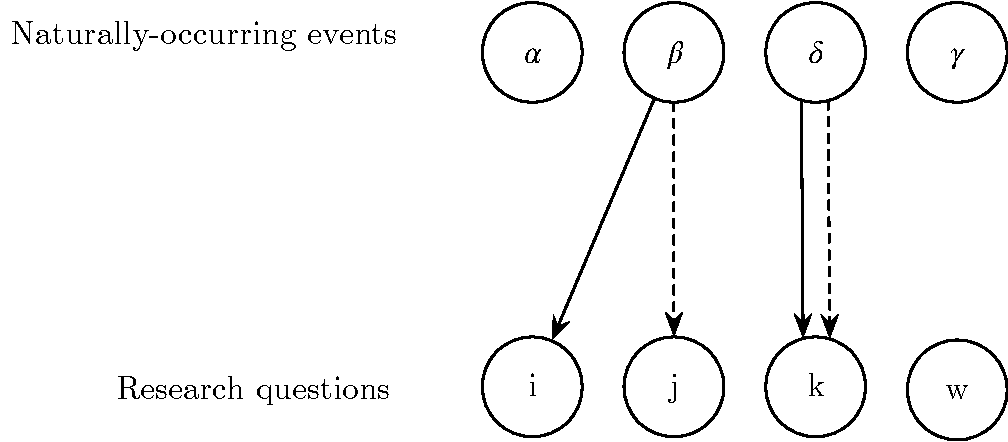
\includegraphics[width=0.7\textwidth]{exhibits/event_rq_mapping.pdf}
  \caption{Exogenous shocks map naturally-occurring events onto 
  research questions via empirical and substantive relevance. Notes:
  
\includegraphics[width=0.075\textwidth]{exhibits/event_rq_mapping_0.pdf}
  = empirical relevance; 
  
\includegraphics[width=0.075\textwidth]{exhibits/event_rq_mapping_1.pdf}
   = substantive relevance.}
  \label{fig:event_rq_mapping}
\end{figure}



\begin{figure}[!htbp]
  %\sffamily
  \centering
  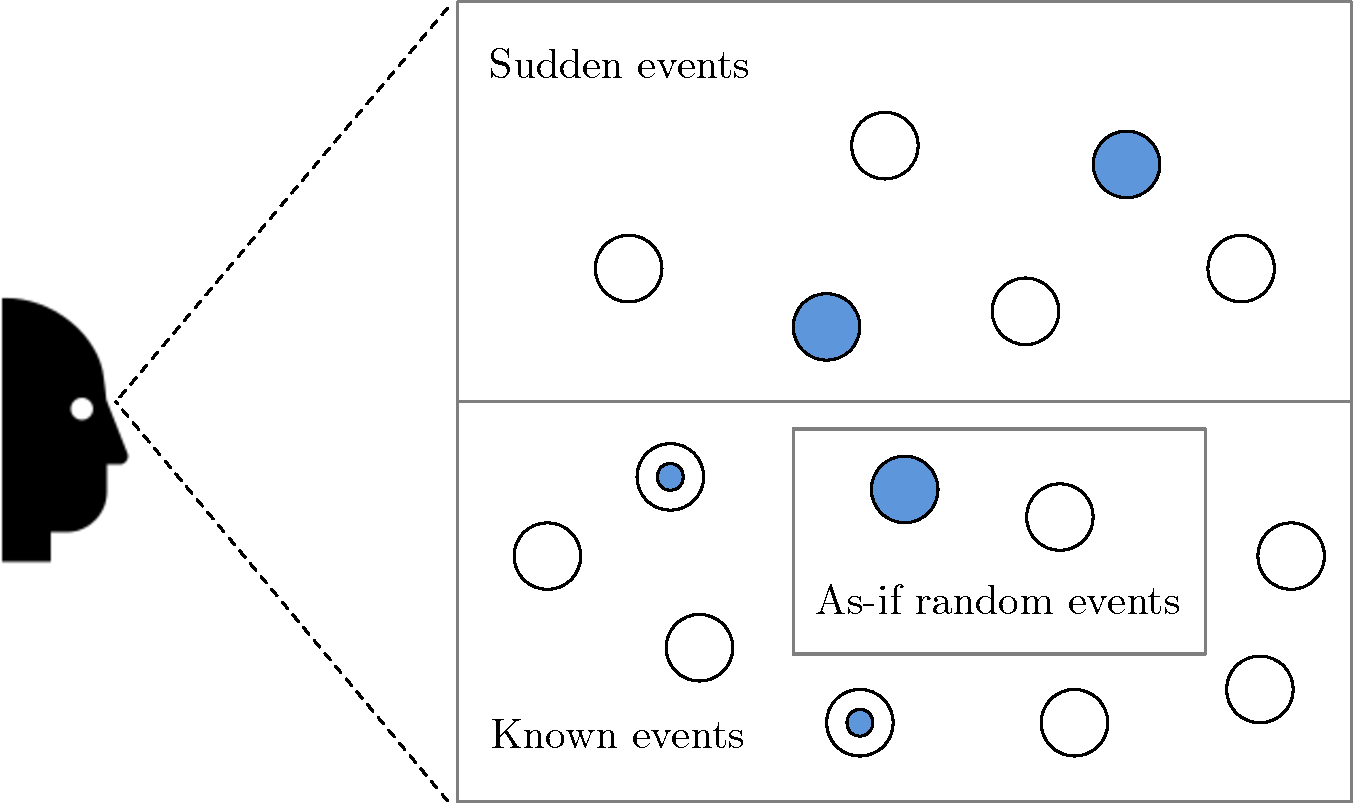
\includegraphics[width=0.75\textwidth]{exhibits/exogenous_shocks_and_ne.pdf}
  \caption{Semantic representation of exogenous shocks in the natural 
  experiment literature. Notes:  
  
\includegraphics[width=0.0175\textwidth]{exhibits/exogenous_shocks_and_ne_0.pdf}
  = exogenous shocks;
  
\includegraphics[width=0.0175\textwidth]{exhibits/exogenous_shocks_and_ne_1.pdf}
  = events that have substantive relevance but do not support causal inference;
  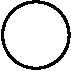
\includegraphics[width=0.0175\textwidth]{exhibits/exogenous_shocks_and_ne_2.pdf}
  = events that lack empirical and substantive relevance.}
  \label{fig:exogeneous_shocks_and_ne}
\end{figure}

\subsection{Exogenous shocks in leadership and management research}
\label{subsec:exogenous_shocks_in_management}

.

\begin{figure}[!htbp]
    %\sffamily
    \normalsize
    \centering
    %
\includegraphics[width=1\textwidth]{exhibits/place_holder.pdf}
    %\input{exhibits/}
    \begin{tikzpicture}
       \begin{axis}[
         width=10cm, height=6cm,
         mark size=3pt,
         xlabel={Counts of studies},
         ytick={0,1,2,3,4,5,6,7},
         yticklabel style={rotate=0},
         yticklabels={
           Academy of Management Journal,
           Journal of Business Ethics,
           Management Science,
           Organization Science,
           Organization Studies,
           Strategic Entrepreneurship Journal,
           Strategic Management Journal,
           Strategic Organization
           },
         axis y line*=left,
         axis x line*=bottom,
         axis line style={draw=none},
       ]
       \addplot + [xcomb] [
           base_c, mark=*, mark options={base_c}
       ] table [x=count, y=journal]{data/articles_by_journal.dat};
     \end{axis}
    \end{tikzpicture}            
    \caption{Distribution of studies that claim to use an exogenous shock across
    management journals.  Notes: N = 32; in the interest of consistency, we
    excluded `exogenous shock' published in Management Science that address
    finance or operations problems. The following journals do not have any
    `exogenous shock' study: Administrative Science Quarterly, Entrepreneurship
    Theory and Practice, Journal of Business Venturing, Journal of Management,
    Leadership Quarterly, Research Policy.}
    \label{fig:studies_across_journals}
\end{figure}         

\begin{figure}[!htbp]
    %\sffamily
    \centering
    
\includegraphics[width=1\textwidth]{exhibits/place_holder.pdf}
    %\begin{tikzpicture}
    \begin{axis}[
      width=12cm, height=4cm,
      mark size=2pt,
      %ylabel={Counts of studies},
      xtick={0,1,2,3,4,5,6,7,8,9,10,11,12,13,14,15,16,17},
      xticklabel style={rotate=90},
      xticklabels={$2002$, $$, $2004$, $$, $2006$, $$, $2008$,
                   $$, $2010$, $$, $2012$, $$, $2014$, $$,
                   $2016$, $$, $2018$, $2019^{*}$},
      axis y line*=left,
      axis x line*=bottom,
      axis line style={draw=none},
    ]
    \addplot + [ycomb] [
        black, mark options={black}
    ] table {exhibits/articles_over_time.dat};
  \end{axis}
\end{tikzpicture}            

    \caption{Classes of events presumed to create exogenous shocks.}
    \label{fig:studies_over_time}
\end{figure}

\begin{sidewaystable}[!htbp]
  \centering
  %\sffamily
  \begin{small}
    \caption{Summary of study events, research questions, and exogenous shocks}
    \vspace{-1.75em}
    \label{tab:}
    \begin{center}
       %\resizebox{1\textwidth}{!}{%
       \begin{tabular}{{@{\extracolsep{2pt}} 
         p{3.75cm}@{\hskip 4mm}   %1 
         p{4.5cm}@{\hskip 4mm}   %2
         p{5.8cm}@{\hskip 4mm}   %3
         p{1cm}@{\hskip 4mm}   %4
         p{1cm}@{\hskip 4mm}   %5
         p{5.8cm}@{\hskip 4mm} %6
         }}
         \toprule \toprule
         & %1
         & %2
         & %3
         \multicolumn{3}{l}{Relevance of the event}\\ \cmidrule{4-6}
         \multicolumn{1}{l}{Study} &
         \multicolumn{1}{l}{Event} &
         \multicolumn{1}{l}{Research question} &
         \multicolumn{1}{c}{Empirical} &
         \multicolumn{1}{c}{Substantive} &
         \multicolumn{1}{l}{Summary}\\
         \midrule \\[-1.8ex]

         Cai \& Shi \parencite*{cai2019159} \dotfill &
         \quad Revelation of the sex abuse of children by Catholic priests in U.S. &
         \quad Does a firm's religious environment influences outside parties' 
         perceptions in contracting with the firm? &
         \multicolumn{1}{c}{$\bullet$} &
         \multicolumn{1}{c}{$\circ$} &
         \quad Revelation of the sex abuse of children by Catholic priests is an
         exogenous shock to the religiosity of a region, which  can meaningfully
         influence the capital structure, credit rating, cost of debt, and
         covenants of firms located in the region.\\ \\

         Gupta et al. \parencite*{gupta2020802}\dotfill &
         \quad Sarbanes-Oxley Act (SOX) \& Global Financial Crisis &
         \quad Does CFO gender influence the likelihood of financial misreporting? &
         \multicolumn{1}{c}{$\bullet$} &
         \multicolumn{1}{c}{$\circ$} &
         \quad The authors expect: i) SOX to lead to a larger decrease in financial
         misreporting for male CFO firms than female-CFO firm; ii) firms to face
         greater pressure to report favorable earnings during crisis periods,
         which is more likely to influence male compared to female CFOs (based
         on the logic that female CFOs will be less likely to engage in fraud
         regardless of stakeholder pressure).\\  \\
         
         Seebeck \& Vetter \parencite*{seebeck2021}\dotfill &
         \quad Brexit Referendum &
         \quad Does board gender diversity affect corporate risk disclosure? &
         \multicolumn{1}{c}{$\bullet$} &
         \multicolumn{1}{c}{$\circ$} &
         \quad The outcome of Brexit Referendum increases the amount of risk
         environment for all UK-based companies, which attenuates reverse
         causality concerns regarding board gender diversity on corporate and
         risk disclosure. \\ \\
         \bottomrule
       \end{tabular}
       %} 
    \end{center}
  \end{small}
\end{sidewaystable}

\begin{sidewaystable}[!htbp]
  \centering
  %\sffamily
  \begin{small}
    \caption*{\textsc{Table I} (cont'd)}
    \vspace{-1.75em}
    \label{tab:}
    \begin{center}
       %\resizebox{1\textwidth}{!}{%
       \begin{tabular}{{@{\extracolsep{2pt}} 
         p{3.25cm}@{\hskip 4mm}   %1 
         p{4.5cm}@{\hskip 4mm}   %2
         p{6cm}@{\hskip 4mm}   %3
         p{1cm}@{\hskip 4mm}   %4
         p{1cm}@{\hskip 4mm}   %5
         p{6cm}@{\hskip 4mm} %6
         }}
         \toprule \toprule
         & %1
         & %2
         & %3
         \multicolumn{3}{l}{Relevance of the event}\\ \cmidrule{4-6}
         \multicolumn{1}{l}{Study} &
         \multicolumn{1}{l}{Event} &
         \multicolumn{1}{l}{Research question} &
         \multicolumn{1}{c}{Empirical} &
         \multicolumn{1}{c}{Substantive} &
         \multicolumn{1}{l}{Summary}\\
         \midrule \\[-1.8ex]
         Vergne \parencite*{vergne20121027}\dotfill &
         \quad 9.11 &
         \quad Does straddling multiple product-market categories dilute stakeholder 
         attention to the stigma of operating in the global army industry?&
         \multicolumn{1}{c}{$\bullet$} &
         \multicolumn{1}{c}{$\bullet$} &
         \quad \textit{``Because the attackers used commercial airlines hijacked by terrorists
         armed with kitchen knives, the definition of the weapons category was
         questioned in the post-9/11 period.''} Hence, 9/11 allows the author to
         test whether the salience of the category `weapons' weakens the negative
         relationship between stigma dilution (i.e., the situation in which a
         diversified business operates also in a stigmatized sector, such as
         `arms') and media disapproval.\\ \\[-1.8ex]
         \dotfill &
         . &
         . &
         \multicolumn{1}{c}{$\bullet$} &
         \multicolumn{1}{c}{$\bullet$} &
         .\\
         \bottomrule
       \end{tabular}
       %} 
    \end{center}
  \end{small}
\end{sidewaystable}


\section{How do exogenous shock differ?}
\label{sec:how_exogenous_shocks_differ}

.

\begin{figure}[!htbp]
  
\includegraphics[width=1\textwidth]{exhibits/place_holder.pdf}
  \caption{A typology of exogenous shocks.}
  \label{fig:exogeneous_shocks_types}
\end{figure}

\section{Harnessing exogenous shocks: opportunities and challenges}
\label{sec:how_exogenous_shocks_differ}

.

\begin{figure}[!htbp]
  
\includegraphics[width=1\textwidth]{exhibits/place_holder.pdf}
  \caption{A decision tree to harnessing exogenous shocks.}
  \label{fig:harnessing_exogeneous_shocks}
\end{figure}

\section{Coda}
\label{sec:coda}
.

%% --------------------------- Bibliography ---------------------------------
%\bibliographystyle{plainnat}
\section{References}
\printbibliography[heading=none]
\end{refsection}

% -------------------------- Appendix --------------------------------------
%\begin{refsection}[references/sample.bib]
%
%\section{Appendix A --- Sample of studies}
%\label{sec:sampling}
%
%\setcounter{table}{0}
%\renewcommand{\thetable}{A\arabic{table}}
%\renewcommand{\thefigure}{A\arabic{figure}}
%
%!! Describe literature search !!
%
%\subsection{References}
%
%\printbibliography[heading=none]
%
%\end{refsection}

% ----------------------------- Closing ------------------------------------
\end{document}